\chapter{Back Ground}

\section{Concurrent Games}
A {\em concurrent game} is played by many agents 
that make their moves concurrently.  
Such a game can be formalized \label{reply1.be.formalized} with the following definition.  

\begin{definition}
A concurrent game graph is a tuple 
$A=\langle m,Q,r,P,\lambda,R,\Delta,\delta\rangle$
with the following restrictions.
\begin{list1}
\item 
	$m$ is the number of agents in the game.
\item 
	$Q$ is a finite set of states.
\item 
	$r\in Q$ is the {\em initial state} of $A$.
\item 
	$P$ is a finite set of atomic propositions.
\item Function 
	$\lambda:Q\mapsto 2^P$ labels each 
	state in $Q$ with a set of atomic propositions.
\item 
	$R\subseteq Q\times Q$ is the set of transitions.
\item 
	$\Delta$ is a set of tokens that can be issued 
	by the agents during transitions.  
\item 
	$\delta:(R\times [1,m])\mapsto \Delta$ is a function that specifies the
    token (move symbol) issued by each agent in a transition.
\end{list1}
\end{definition} 
During a transition, each agent selects a token.  
If there is no transition matching all the tokens selected by the agents, 
then there is no transition.  
Otherwise, the matching transition takes place.  
\qed 


In Figure~\ref{fig.cg}, we have the graphical representation of a concurrent game graph.  
\begin{figure}[!ht]
\begin{center}
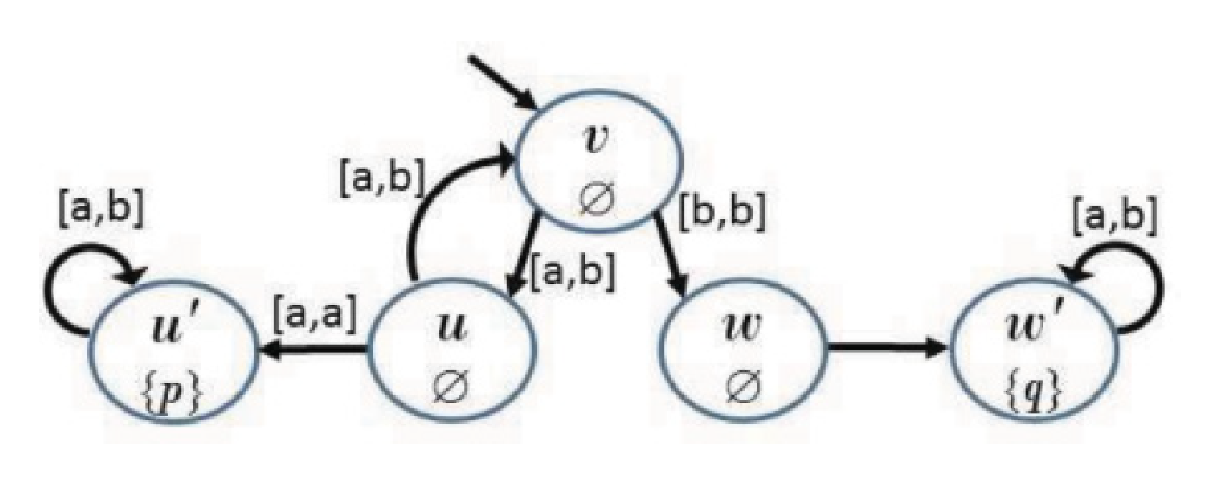
\epsfig{file=cg.eps,width=80mm} 
\end{center}
\caption{A concurrent game graph}
\label{fig.cg}
\end{figure} 
The ovals represent states while the arcs represent 
state transitions.  
We also put down the $\lambda$ values inside the corresponding states. 
On each edge, we label the tokens issued by the agents. 
Specifically, the label on arrow $(q,q')$ is 
$[\delta((q,q'),1),\ldots,\delta((q,q'),m)]$.  
For example, in Figure~\ref{fig.cg}, 
on edge $(v,u)$, we have label $[a,b]$ meaning that 
to make the transition, agent 1 has to choose token $a$ while 
agent 2 has to choose $b$.  

For convenience, in the remaining part of the manuscript, we assume that we are always in the context of a given game graph $\calg=\langle m,Q,r,P,\lambda,R,\Delta,\delta\rangle$.
Thus, when we write $Q,r,P,\lambda,R,\Delta$, and $\delta$ we respectively refer to the corresponding components of this $\calg$.  

A {\em state predicate} of $P$ is a Boolean combination of elements in $P$.
% We let $\emstp(P)$ be the set of state predicates of $P$.
The satisfaction of a state predicate $\eta$ at a state $q$,
in symbols $q\models \eta$, is defined in the standard way.

A {\em play} is an infinite path in a game graph.
A play is {\em initial} if it begins with the initial state.
Given a play $\rho=\bar{q}_0\bar{q}_1\ldots$,
for every $k\geq 0$, we let $\rho(k)=\bar{q}_k$.
Also, given $h\leq k$,
we let $\rho[h,k]$ denote $\rho(h)\ldots\rho(k)$ and
$\rho[h,\infty)$ denote the infinite tail of $\rho$
from $\rho(h)$.
A {\em play prefix} is a finite segment of a play from the beginning of
the play.
Given a play prefix $\rho=\bar{q}_0\bar{q}_1\ldots \bar{q}_n$, 
we use $|\rho|=n+1$ for the {\em length} of $\rho$.
For convenience, we use $\emlast(\rho)$ to denote the 
last state in $\rho$, i.e., $\rho(|\rho|-1)$.  

Let $Q^*$ be the set of finite sequences of states in $Q$.  
For an agent $a\in [1,m]$,
a {\em strategy} $\sigma$ for $a$ is
a function from $Q^*$ to $\Delta$.
An {\em agency} $A$ of $[1,m]$ is an integer subset of $[1,m]$.  
For example, ``$\{1,3,4\}$'' represents the agency that consists of agents 1, 3, and 4. 
A {\em strategy profile} (or {\em S-profile}) $\Sigma$ of 
an agency $A\subseteq [1,m]$ 
is a partial function from $[1,m]$ to the set of strategies
such that, for every $a\in[1,m]$, 
$a\in A$ iff %\footnote{``{\em iff}" is a shorthand for ``{\em if and only if}."} 
$\Sigma(a)$ is defined.  
The composition of two S-profiles $\Sigma,\Pi$,
in symbols $\Sigma\circ\Pi$, is defined with
the following restrictions for every $a\in[1,m]$.
\begin{list1}
\item If $\Pi(a)$ is defined,
    then $\Sigma\circ\Pi(a)=\Pi(a)$.
\item If $\Sigma(a)$ is defined and $\Pi(a)$ is undefined,
    then $\Sigma\circ\Pi(a)=\Sigma(a)$.
\item If $\Sigma(a)$ and $\Pi(a)$ are both undefined,
    then $\Sigma\circ\Pi(a)$ is also undefined.
\end{list1} 
% Later, w
We will use composition of S-profiles to model 
inheritance of strategy bindings from ancestor formulas. 

A play $\rho$ is compatible with a strategy
$\sigma$ of an agent $a\in [1,m]$
iff for every $k\in [0,\infty)$,
$\delta((\rho(k),\rho(k+1)),a)=\sigma(\rho[0,k])$.
The play is compatible with an S-profile $\Sigma$ of agency $A$ iff for every $a\in A$, the play is compatible with $\Sigma(a)$ of agent $a$.

\section{Turn-Based Games}
Another popular game structure is {\em turn-based game} in which at each state, at most one agent gets to decide the next state.
For example, in figure~\ref{fig.tg}, we have the graphical representation of a turn-based game graph with initial state $v$.
\begin{figure}[!ht]
\begin{center}
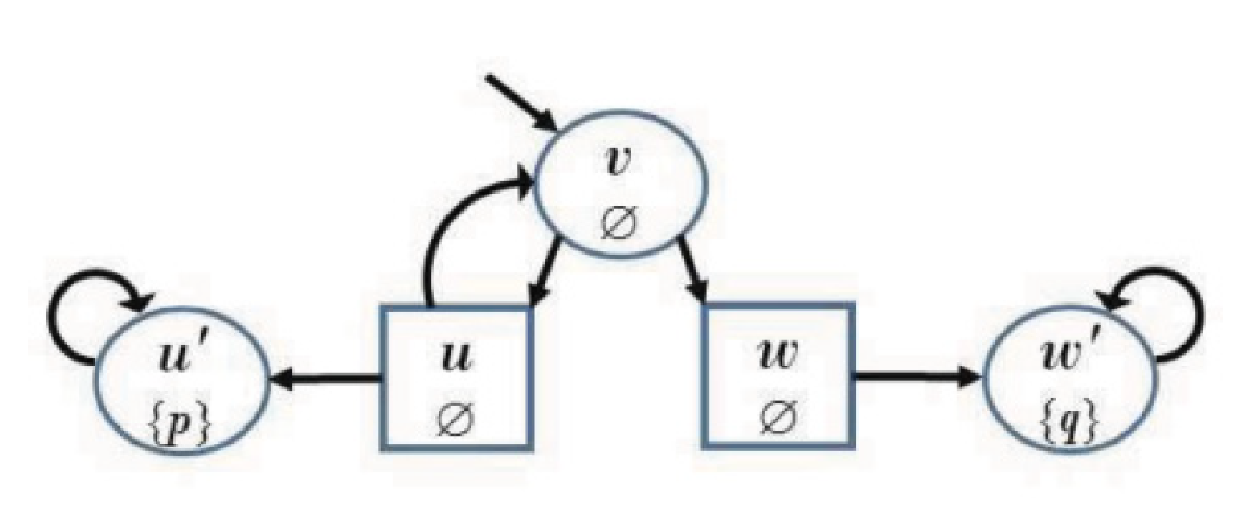
\epsfig{file=tg.eps,width=80mm} \\
$\bigcirc$ belongs to Agent 1 and $\pfrr$ belongs to Agent 2.
\end{center}
\caption{A turn-based game graph}
\label{fig.tg}
\end{figure} 
The ovals and squares represent states respectively of gent 1 and agent 2.
The arcs represent state transitions.  

In fact, every turn-based game can be represented as a special case of 
concurrent games.  
Specifically, a turn-based game 
$\calg=\langle m,Q,r,P,\lambda,E,\Delta,\delta\rangle$ 
can be viewed as a concurrent game with the following restrictions. 
\begin{list1} 
\item $\Delta=Q\cup\{\perp\}$ where $\perp$ denotes a dummy move not in $Q$. 
\item For every $(q,q')\in R$, if $q$ belongs to agent $a$, 
	then $\delta((q,q'),a)=q'$ and 
	for every $a'\neq a$, $\delta((q,q'),a')=\perp$. 
\item For every $(q_1,q_2),(q_3,q_4)\in R$ and agent $a$, 
	$\delta((q_1,q_2),a)=\perp$ if and only if $\delta((q_3,q_4),a)=\perp$.  
	This restriction says that every state can be owned by only one agent. 
\end{list1} 
For convenience, for a turn-based game, the owner of a state $q$, $\omega(q)$ in symbols, is defined as agent $a$ with $\forall (q,q')\in E(\delta((q,q'),a)=q'$.  
For ease of notation, we denote with $Q_a = \{q \in Q \mid \omega(q)=a\}$ the states owned by an agent $a$.

In the investigation of many research issues, turn-based game graphs are easier to handle than concurrent game graphs.   
So in latter sections, we sometimes use turn-based game graphs in examples and explanation of the theory as we see fit.

\section{Two-player concurrent game structures}
To facilitate the explanation of resilience analysis in a game's perspective, we start by defining a special case of the concurrent game, $\calk=\langle 2,Q,r,P,\lambda,R,E_1,E_2,\delta\rangle$.
The first difference is that there are only 2 players in the game.
For convenience, we divide the token set that player can choose, $\Delta$, into 2 subsets $E_1$ and $E_2$.
Intuitively, $E_1$ are the tokens set that can be picked by protagonist and $E_2$ are the tokens set that can be picked by antagonist.
Moreover, each member of $E_2$ are labelled by either $error$ or $non-error$ moves.

\section{Fault Tolerance}
Resilience to errors in computer systems is usually achieved through error recovery design as illustrated in Figure~\ref{fig.frwk}.  
\begin{figure}[t]
\begin{center}
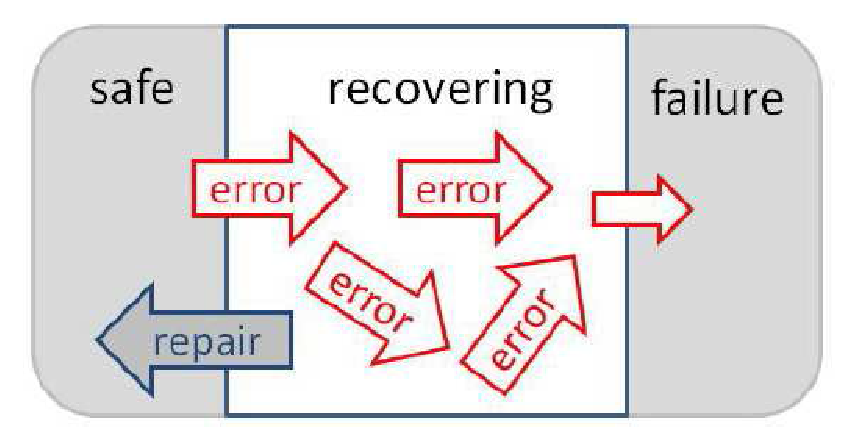
\epsfig{file=frwk.eps,width=60mm}
\caption{Framework of resilience design}
\label{fig.frwk} 
\end{center}
\end{figure}
The system states can be partitioned into three regions safe, recovery, and failure. 
The left part of the figure represents the safety region.
The states in this region represent those for 'normal' operation. 
When an error occurs, the system goes through a recovery process, in which it follows some recovery mechanism.
This is shown as the "recovering" area in Figure~\ref{fig.frwk}.
In this region, the system tries to repair the effects caused by an error and thus to go back to the safety region. 

In the recovery region, however, errors may still happen.
In general, fault-tolerant systems are built under the assumption that error detection and recovery is speedy and that there can only be a few errors during the process of recovery.
If the recovery mechanism is not resilient enough, a few errors may drive the system into failure.  

We use following 3 examples from computer architecture, OS interrupt handler and security system to illustrate our point. 

\begin{example} 
{\bf (Fault-tolerant computer architectures):}  
\label{exmp.avi}
In computer architectures, fault-tolerance is usually achieved via hardware duplication.  
Consider an example of a multi-processor system that includes $n$ processor copies and $m$ memory copies.  
The $n$ processors each can follow the instructions of the original system, or be engaged in memory recovery. 
When a copy of the memory fails, a processor can be assigned to recover it.
Majority check can be used to detect that a processor is faulty or that memory copy is faulty (often, both would happen at the same time).
For recovery, we can set a free processor to recover some memory copy, or make a processor follow the code of the majority of processors.

The key to error resilience is to decide whether to make a processor follow the execution of the majority, or to assign it to recover faulty memory.
If too many errors occur in a short while before the errors can be recovered from, then there may be no more processors left to carry out any more recovery. 
When such a critical situation arises, the system enters failure state when another error is induced.  

The recovery mechanism described above is typical in the design of fault-tolerant systems \cite{Pradhan96}.  
As explained, a practical recovery mechanism usually does not rely on the detailed structure of the system.  
Instead, error-detection techniques such as parity checks, voting (for majority checks), etc., are usually employed.  
In fact, the number of duplicates is usually critical to the resilience of the system to errors.
As long as the majority of the duplicate modules can be recovered in time (i.e., before the next wave of errors), resilience of the system can be achieved. 
\qed 
\end{example} 

\begin{example} {\bf (Exception handling):} 
\label{exmp.ehan} 
At the operating system level, errors are usually signalled via interrupt lines and handled with routines called handlers.
The first thing that needs to be done by a handler is to save the CPU state of the interrupted process.
In some operating systems, a static memory space is used for this purpose for each handler. 
In such a scheme, if the same error happens again while executing the error handler, then the system can run into the risk that the CPU states of the interrupted handler can be overwritten and destroyed. 

Another scheme is to use a stack to save the CPU states of the interrupted processes.  
Such a scheme seems resilient to errors that happen during the execution of error handlers.
Still, too many errors that happen during the execution of error handlers
can deny critical functions of the system and incur failures, including missed timer updates and priority inversions.
Thus, a proper assumption on the timely error recovery by the error handling routines is critical to the design of 
error resilience in such cases.
\qed 
\end{example} 

\begin{example} {\bf (Security attacks):}
\label{exmp.satt}
Security in the Internet also relies on resilience to attacks of hackers, viruses, malware, etc.  
For example, one common technique of attacks to communication modules is to overflow the communication buffers.  
In such attacks, the sizes of the buffers and the ability of the security procedures to detect and recover from such overflowing attacks is crucial to the resilience design.  
\qed 
\end{example} 

These examples show that recovery is a crucial concept for designing systems that are resilient to errors. 
When system errors are detected in such a system, the system activates a recovery mechanism to remove the effect of the errors.
When designing such systems, the system designers usually know what errors and failures the systems can expect, according to the specification.
To avoid failures in the occurrence of dense errors, the system designers usually incorporate many error recovery mechanism in the system, e.g., exception handlers and hardware/software redundancy. 
But, in general, it would be difficult for the designers to evaluate how effective their recovery mechanism is to dense errors.
To overcome this difficulty, we believe that it is important to support them with automated analytical tools with a solid foundation.

Resilience has also been used in \cite{EhlersT14,BloemEJK14} with a similar goal.
When synthesising code, one relies on assumptions of the behavior of the environment, and the formal specification would only ask for the provision of guarantees under the condition that the assumptions are satisfied.
When evaluating the quality of an implementation, the behavior in cases where the environment does not comply with the assumption matters.
In \cite{EhlersT14,BloemEJK14}, the resilience model we have introduced in the conference version \cite{HPSW/12/rapidRecovery} of this paper has been followed up upon, and proven to be well suited for reactive synthesis.

In this work, we use these observations to design a theoretical framework for synthesizing a control mechanism that provides the maximal resilience against software errors in a realistic error model.

 